% Prespecification, validation gate and execution record (Section S4).
% Moved from sections/supplement.tex and sections/results.tex of the
% rule-assembled attempt and reorganized during the journal revision
% (agent S, 2026-10-13). Claim markers (SUPxx, Mxx, RCxx) refer to rows in
% claim-evidence.md. Sentences marked as read after the results became
% available are post-release readings.

This section is the audit record of the prespecified design: how the protocol came to be (Section~\ref{sec:record-history}), what had been seen before the confirmatory run (Section~\ref{sec:record-exposure}), the validation gate that had to pass first (Section~\ref{sec:record-gate}), the execution and release of the run, including amendment v4.4 (Section~\ref{sec:record-execution}), and who approved what (Section~\ref{sec:record-governance}). Table~\ref{tab:record-identifiers} lists the identifiers of the frozen and successor records, so that the prose does not repeat them.

Here, prespecified means frozen in the project repository before the confirmatory run, by a Git revision and a freeze record that binds the protocol, criteria, inventory, seeds, environment and code by SHA-256; no public preregistration exists. The archive holds these records, so a reader can check that the archived protocol and code match the hashes bound in the freeze records. Four bound files are archived only as redacted copies: two files of the frozen code closure (a verification script and an integration test), the record of revision v4.1 and the anchor's reliability module. For these four, the check rests on the original SHA-256 digests recorded in the archived \code{plan.json}. Some other bound files are not archived at all: the v1 freeze record also binds earlier versions of two code files and the validation, review and authority records of v1, and the freeze record of SHP successor 1 binds the anchor's unit tests. Hashes bind the content of a record, not the time at which it was written: the prespecification records carry no external timestamp, and the dates of the events below rest on the repository history and the project's records.

\begin{table}[htbp]
\caption{Identifiers of the frozen and successor records cited in this section. SHA-256 digests are given in full; the archive holds every record}\label{tab:record-identifiers}
\centering\footnotesize
\begin{tabular}{@{}>{\raggedright\arraybackslash}p{0.29\textwidth}>{\raggedright\arraybackslash}p{0.4\textwidth}>{\raggedright\arraybackslash}p{0.23\textwidth}@{}}
\toprule
Record & Identifier & Role \\
\midrule
v1 protocol & Git revision \texttt{fd65d2a}; SHA-256 \texttt{fb6b4dcf4316}\allowbreak\texttt{1a52c725e565}\allowbreak\texttt{bf2a4d269742}\allowbreak\texttt{3bec7d138ad1}\allowbreak\texttt{d30388547cfc}\allowbreak\texttt{d706} & first frozen protocol \\
v4 freeze record & Git revision \texttt{37513841}; SHA-256 \texttt{99c4277235d4}\allowbreak\texttt{f2303b6f009d}\allowbreak\texttt{6ead8287a5d7}\allowbreak\texttt{1372744dd678}\allowbreak\texttt{1e1e2d184771}\allowbreak\texttt{0837} & frozen protocol of the run \\
code closure bound by the v4 freeze record & SHA-256 \texttt{db9d6eadb5019d69}\allowbreak\texttt{1a8c73703d511d03}\allowbreak\texttt{37dc49834bb219d1}\allowbreak\texttt{68a27693df0e0acd} & frozen scientific code \\
G1c successor record & SHA-256 \texttt{a945e848}\allowbreak\texttt{4791f886}\allowbreak\texttt{289d51b0}\allowbreak\texttt{83886854}\allowbreak\texttt{b4f540f6}\allowbreak\texttt{b26dcf14}\allowbreak\texttt{63d8d4c9}\allowbreak\texttt{dcd9a4d6} & repaired G1c summary \\
release amendment & Git revision \texttt{428ca7cd} & release on completion \\
release wrapper & introduced at Git revision \texttt{1f74e902}; SHA-256 \texttt{9acdfcdd}\allowbreak\texttt{077daa73}\allowbreak\texttt{e2c18999}\allowbreak\texttt{5317ae28}\allowbreak\texttt{e405b202}\allowbreak\texttt{f66cc024}\allowbreak\texttt{3566d902}\allowbreak\texttt{bca5a0c1}; the release record binds the hash of the revised version that ran, archived from Git revision \texttt{9669b509} & implements the release rule \\
amendment v4.4 & own freeze record, status \texttt{frozen}, approved 1 October 2026 at 14:33 UTC & propagation gaps \\
SHP successor 1 & code revision \texttt{17a0dbed}, frozen 28 September 2026 at 07:51:17 UTC & reliability anchor \\
\botrule
\end{tabular}
\end{table}

\subsection{Prespecification and protocol history}\label{sec:record-history}\phantomsection\label{supp:protocol-lineage}

The first protocol, v1, was frozen on 25 September 2026 (Table~\ref{tab:record-identifiers}). % M48
Its zero-strength coverage check failed operationally and numerically: no full 81-cell repetition completed under the fixed time cap, 14 of 40 refits in a cost probe failed matching, and coverage was therefore not estimated. % M49
The report also raised a second caveat at $a=0$: the influence arm transported normal ranks every wave, while the v1 version of B generated a stationary Gaussian autoregressive law matched only at lags one and two. The code did not establish that the two finite-$N$ laws were equal. % M49
Two exploratory amendment proposals followed the same day (Proposals A and B; not adopted). The linked successor, v4, changes those laws, the profile fit, the nuisance calculation and the validation gates while preserving the v1 protocol bytes and historical outputs. % M50
Its decision specification (items D1--D11) was revised as v4.1 (items R1--R8) and implemented in the amendment text v4.3, together with the decisions taken on two independent reviews of the implementation; v4.2 is an intermediate revision preserved by hash (Table~\ref{tab:glossary-versions}). The v4 freeze record was written at Git revision \texttt{37513841} before any gate stage ran. % M51
The hash-bound amendment text predates its own freeze record. Its immutable bytes still say that no v4 freeze exists; the freeze record, whose status is \texttt{frozen}, controls. % M81
The decision specification allowed optional shards on other hosts. The amendment permits additional shards only with the same code and numerical equivalence and binds eight local shards, as does the later review decision taken after the first author dropped multi-host execution. The freeze record fixes eight shards; a host-equivalence check also failed (Section~\ref{sec:verification}). % M82

The frozen G1c aggregate returned a NumPy boolean that the runner could not serialize into its complete summary line. % M86 RC38
A successor record stores that summary outside the seal, computed by the frozen aggregating function (Table~\ref{tab:record-identifiers}); this repairs the summary record and changes no gate criterion. % M86 RC39
The later report loader checks the successor's freeze binding, store identifier and completed-task count. It requires the successor's pass to equal the frozen G1c predicate applied to its own fields. It accepts only the digest recorded when the successor was produced and uses the successor only when the sealed criteria log lacks a complete summary. % M86 RC40
The later release wrapper and reporting loader lie outside the frozen scientific code closure. Two later amendments are linked to the freeze without editing it: the release amendment of 28 September 2026 and the operational amendment v4.4 of 1 October 2026 (Section~\ref{sec:record-execution}). % M85 M86

\subsection{Order of events and cumulative exposure}\label{sec:record-exposure}

Table~\ref{tab:record-events} gives the order of the events that matter for how confirmatory the results are. Exposure is cumulative: every result seen before the run counts, whatever the law, algorithm or sample size that produced it. % M52

\begin{table}[htbp]
\caption{Order of events, from the first positive-strength results to the journal revision. Exposures concern the laws, algorithms and sizes named in each row}\label{tab:record-events}
\centering\footnotesize
\begin{tabular}{@{}p{0.18\textwidth}p{0.75\textwidth}@{}}
\toprule
Date (2026) & Event and what was seen \\
\midrule
24 September & Pilots of an earlier design (a different generator with a fixed strength of 0.4, an older autoregressive comparison and other features): classification non-degeneracy gates at $r=0.65$ and 0.70, and a strength selection that used classification at $r=0.80$. Together with the single bit of the next row, these are the results that v1 declares as prior exposure. \\
24--25 September & Draft protocol under decision 14 fixes the AUC target 0.70 (secondary targets 0.60 and 0.80), the strength grid and the regions small ($0<a^*\le0.03$) and large; its text records that the 0.03 cut was fixed before its pilot. The pilot reveals a single bit: whether the pilot boundary at $r=0.70$ lies inside the grid. \\
25 September & v1 frozen with the same target, grid and cut. Its zero-strength coverage check fails. \\
25 September & Probes of v1 and of the two proposals at $r=0.70$, under their own laws: positive-strength AUCs (v1 interior probe; Proposal A at $a=0.10$ and 0.03) and Proposal B's positive-strength matching quantities. \\
25 September & v4 decided, revised and implemented; frozen before any gate stage, keeping the AUC target, the 0.03 cut, the discriminator's shrinkage and the parameter box of v1 (Table~\ref{tab:design-conventions}). \\
27--28 September & Docking studies compute AUCs under the v4 law at reduced sizes in two cells, and a timing probe prints mean lag correlations of 50 project panels in two cells (Section~\ref{sec:verification}). \\
28 September & G1c summary repaired by its successor record (07:14 UTC); exploratory analyses X1--X2 and X3--X7 declared; SHP successor 1 frozen (07:51 UTC); release amendment registered (23:28 UTC) with the gate at its fourth stage and no tier started. \\
28--30 September & Exploratory analyses X1a, X1b, X2 and X5 run and are read, as their declarations allow; X3, X4, X6 and X7 run and stay sealed. \\
30 September & All five recorded gate stages passed; the tiers start (decision log item 114). \\
1 October & Shard 5 stops during tier 2 (04:18 UTC); amendment v4.4 approved by the first author and the eight shards relaunched (14:33 UTC); ratification of delegated decisions and amendments (decision log item 161). \\
8 October & The results become available on completion of the full inventory (Section~\ref{sec:record-execution}). \\
8--9 October & The assembled text with the released values is read; the wording of the pre-written blocks is corrected in two recorded batches and re-pinned, with rule identities, conditions, slots, order, values and readings unchanged; the rule-assembled record is produced on 9 October (Section~\ref{sec:rule-record}). \\
9--13 October & AI reviews of the rule-assembled PDF; the journal revision begins on 13 October (Section~\ref{sec:rule-record}). \\
\botrule
\end{tabular}
\end{table}

\paragraph{When the target and the cut were fixed.}
The primary target AUC 0.70 and the 0.03 cut between the small and large regions were written into the draft protocol under decision 14 and frozen unchanged in v1 and v4; the records give no further rationale for their values (Table~\ref{tab:design-conventions}). At that point, the positive-strength results declared as prior exposure were the classification gates and the strength selection of the earlier design, which used another generator, strength, comparison and set of features. Under the draft design, its pilot exposed one bit, whether the boundary at $r=0.70$ was inside the grid. Positive-strength AUCs of designs close to the final one came after the target and cut were fixed: after the v1 freeze, the v1 interior probe at $(a,r)=(0.30,0.70)$ gave a conditional reference AUC of \resultnum{j.exposure.v1_probe_auc}{0.944}, and Proposal A's loose-acceptance calibration at $r=0.70$ gave a mean AUC of \resultnum{j.exposure.proposal_a.a010.mean}{0.756} over 40 refits at $a=0.10$ (range \resultnum{j.exposure.proposal_a.a010.min}{0.732}--\resultnum{j.exposure.proposal_a.a010.max}{0.790}) and \resultnum{j.exposure.proposal_a.a003}{0.589} in one probe at $a=0.03$. Read after the results became available: those two values bracket the target between $a=0.03$ and 0.10 at $r=0.70$, so they anticipated the released first boundary of \resultnum{j.b.r070.first.point}{0.10} and its large-region label at that share, under a different law and a looser acceptance rule. % SUP10 M52

\paragraph{Exposure inventory.}
Before v1, balanced-accuracy gates at $r=0.65$ and 0.70, an earlier choice at 0.80, and an interiority bit at 0.70 were seen. % M52
Later v1 and Proposal A probes exposed zero-strength refit AUCs, an interior AUC and positive-strength AUCs at $r=0.70$; Proposal B exposed positive-strength matching quantities. % M52
Twenty-six valid zero-strength v1 refits at $r=0.70$ averaged 0.530. % SUP10
After the v4 freeze, the model docking study computed mean discriminator AUCs under the v4 law with fitted B at $(a,r)=(0.30,0.70)$ and $(0.03,0.50)$, with $N=1{,}002$, 100 training and 250 test networks per class and 50 replicates. Before its comparison plan was committed, a timing probe printed mean $L_1$--$L_5$ of 50 project panels in two cells. The docking means were 0.677 at $(0.30,0.70)$ in both implementations and 0.506 and 0.507 at $(0.03,0.50)$. At these reduced sizes they are not estimates of the study estimand, and they are disclosed only because exposure is cumulative. % M84 SUP10
The gate criteria and their values (Section~\ref{sec:record-gate}) were also seen before the tiers ran. The exploratory analyses X1a, X1b, X2 and X5 were read before the results became available, as their declarations allow: X5 runs only at zero strength, and X1a, X1b and X2 compare the influence arm with a mean-field twin, the twin with B, or measure the drift on latent paths, so none estimates the confirmatory curve. X3, X4, X6 and X7, which use the confirmatory cells against B, stayed sealed until the results became available (Section~\ref{sec:exploratory}).
These historical values document cumulative exposure; they do not determine the v4 curve, because the law and the algorithm changed and nothing constrains the AUC to be monotone across the grid (decision item D8). They mean that $r=0.70$ was examined during calibration, and that the global method was chosen after partial exposure; evaluation on new seeds of this amended protocol is therefore not a fully blind confirmation. The whole curve stays the primary result, with the provenance of each $r$ shown, and the other eight shares are not promoted to a new primary set. % M52 M53

\subsection{Validation gate}\label{sec:record-gate}\phantomsection\label{supp:gate-accounting}

\paragraph{Stages and criteria.}
The zero-strength fitting check (G0) audits eight grids without reporting parameters or AUCs; all identity-model zero-strength fits must be anchor-exact, no fit may exhaust its budget, and implementation-status gaps may occupy at most 1\%. The G0 implementation-status ratio counts statuses over all attempts, retries included, and divides by the number of fits. % SUP07 M37
The identity unit tests (G1a) test full-population byte identity in the declared channels and zero local variance at the anchor. The band calibration on synthetic scores (G1b) tests five synthetic-score scenarios with 1,000 repetitions each and requires at least 935 joint covers in each. The zero-strength band check (G1c) runs 50 zero-strength pipelines at each of three signal shares; every fit must be anchor-exact, at most three of 150 pointwise intervals may miss 0.5, and the mean AUC must remain within three standard errors of 0.5. A failed stage requires a documented amendment. At zero strength the persistence models with an identity have no matching discrepancy by construction, and G1b uses zero nuisance variance, so these zero-strength checks cannot detect positive-strength matching bias. % SUP07 M38 M39

The positive-strength dispersion check (G2) uses 100 independent pipelines in each of seven declared cells, grouped into 50 disjoint pairs. It compares the empirical variance of paired logit differences with the reported variance of those differences and checks the median $V_{\mathrm{nuis}}(0.005)/V_{\mathrm{nuis}}(0.01)$ in each cell against $[0.8,1.25]$. At most five technical failures per 100 in a cell and 14 per 700 pooled are allowed; failed pairs leave only the ratio calculation and remain in both failure denominators. The nuisance-variance check (G2c) compares local variance with 100 and 40 full refits in two declared cells. It permits at most three and two failures, respectively. Each refit includes matching, validation and training; its persistence-arm reference is regenerated at the refit parameter using baseline reference seeds, and its influence-arm reference uses fixed seeds. One-sided bootstrap bounds for the local/full-refit variance ratio must not lie wholly below 0.8 or above 2.0. G2c complements G2; G2 alone was calibrated to detect understated uncertainty. These gates do not prove absolute coverage away from zero strength. Their end-to-end tasks use B on the observed channel at the declared cells, without establishing uniform adequacy across all persistence models, channels or sensitivities. % SUP08

\paragraph{Artificial criterion calibration.}\phantomsection\label{supp:gate-calibration}
% SUP16
The archived criteria record binds the calibration script and the criteria code by SHA-256, and the v4 freeze record binds both at revision \texttt{37513841}. Development and verification each used 3,000 artificial experiments with distinct seeds. G2 generated seven independent cells with 100 independent pipelines each: logits were $\ell=\mu_c+0.025T/\sqrt{5.2/3.2}$, with equally spaced $\mu_c\in[-0.2,2]$ and $T\sim t_{5.2}$ (ordinary kurtosis 8), and reported AUC errors were $0.025p(1-p)$ for $p=\mathrm{logit}^{-1}(\ell)$. The leave-one-out diagnostic retained its shared-data dependence. G2c generated 2,000 local draws and 100 or 40 refits from $t_{5.2}$. Independent Bernoulli failures at 1\%, independent of the data, affected each G2 pipeline and G2c refit; failed pairs left only the G2 ratio calculation. Individual finite-difference variance ratios were lognormal with log-mean zero and log-standard deviation 0.25, aggregated by the median within each cell. Each interval used 399 resamples, keeping G2 pairs intact and resampling local draws and refits separately in G2c. Verification compared reported standard-error scales 1, 0.8 and 1.4 against the developed thresholds. This calibration calls neither the panel simulator nor the discriminator. It assumes available local draws from the two G2c baselines and does not model their additional failures; a failed real baseline still blocks G2c. Its operating characteristics apply to this artificial model, not uniformly to the full experimental inventory.
With correct standard errors, the estimated joint pass probability is 95.17\%, with a Monte Carlo error of 0.39 percentage points. Thus, the calibration does not demonstrate that the true probability reaches 0.95. % M77

\paragraph{Binding and stop rule.}
% SUP09
The first freeze record must bind the amendment, code, inventory, criteria, allocation, seeds and environment before gate execution. A second hash-bound record after G0 fixes its blinded status projection, the actual G2 cell list, failure-rate implication and any prerequired recalibration; a projected pass probability below 0.80 stops before G2. Failed stages do not rerun against altered criteria. Gate repetition estimates and AUC-unit mean shifts remain sealed outside Git until confirmatory results are committed. Confirmatory namespaces remain unavailable until all gates pass. Ordered, resumable tiers preserve shard manifests and the four unit statuses at the operational close.
The G0-based stop rule is sharp. In the inference docking's evaluation of the rule (Section~\ref{sec:verification-docking}), one gap among the 54 relevant G0 fits already gives a predictive probability of about 0.445. Thus, a single numerical failure at those cells ends the confirmatory study under the frozen rules. % M78
Seed derivation, the separation of namespaces and the seed audit are described in Section~\ref{sec:dd-seeds}.

\paragraph{Outcomes.}
% Moved from sections/results.tex (Validation gate) of the rule-assembled attempt.
All five recorded stages of the validation gate passed, in the frozen order G0, G1b, G1c, G2, G2c, before any confirmatory seed was derived (Table~\ref{tab:v4-T3}, Fig.~\ref{fig:gate-diagnostics}). The identity unit tests (G1a) are not part of the sealed gate records, and no separate execution record reports their status; the test runs on Linux described in Section~\ref{sec:verification} were made on another platform and are environment diagnostics, not a record of G1a in the bound environment.
In G0, the counts were: \resultnum{v4.gate.G0.anchor_failures}{0} zero-strength identity fits without status \texttt{anchor-exact}; \resultnum{v4.gate.G0.budget_statuses}{0} attempts with status \texttt{budget}; and \resultnum{v4.gate.G0.implementation_statuses}{2} attempts with status \texttt{numerical-limit} or \texttt{ill-conditioned}, across \resultnum{v4.gate.G0.fits}{648} fits. The respective limits were zero, zero and \resultnum{v4.protocol.g0.implementation_limit}{1}\% of fits. G0 published only statuses, counts, residuals in standard-error units and validation outcomes.
In G1b, joint coverage was lowest at \resultnum{v4.gate.G1b.coverage_min}{952} of \resultnum{v4.protocol.g1b.repetitions}{1,000} repetitions across the five synthetic-score scenarios, compared with the pass mark of \resultnum{v4.protocol.g1b.pass_mark}{935}. The empirical max-$t$ critical value exceeded the \resultnum{v4.protocol.critical_floor}{2.7729} floor in \resultnum{v4.gate.G1b.exceeds_floor_count_prose}{1,363} of \resultnum{v4.gate.G1b.completed_prose}{5,000} repetitions.
In G1c, all \resultnum{v4.gate.G1c.anchor_count}{150} zero-strength fits had status \texttt{anchor-exact}. At the \resultnum{v4.protocol.critical_floor}{2.7729} floor, \resultnum{v4.gate.G1c.pointwise_failures}{1} of \resultnum{v4.protocol.g1c.fits}{150} intervals missed \resultnum{v4.protocol.null_auc}{0.5} (limit three). The standardized mean deviation of the AUC from \resultnum{v4.protocol.null_auc}{0.5} was \resultnum{v4.gate.G1c.mean_z}{0.376} (limit \resultnum{v4.protocol.g1c.mean_z_limit}{3}), and the tie rate was \resultnum{v4.gate.G1c.tie_rate}{0.0000}.
In G2, across the \resultnum{v4.gate.G2.n_cells}{7} allocated cells, the pooled ratio of observed to model-implied dispersion of paired logit differences was \resultnum{v4.gate.G2.pooled_ratio}{0.971}, with a bootstrap interval from \resultnum{v4.gate.G2.pooled_lower}{0.760} to \resultnum{v4.gate.G2.pooled_upper}{1.125}. Every cell interval met its calibrated threshold. The cell medians of the finite-difference variance ratio ranged from \resultnum{v4.gate.G2.fd_median_min}{0.951} to \resultnum{v4.gate.G2.fd_median_max}{1.000}, within the required range of \resultnum{v4.protocol.g2.fd_range.lower}{0.8} to \resultnum{v4.protocol.g2.fd_range.upper}{1.25}. The technical-failure count was \resultnum{v4.gate.G2.failures}{0} among \resultnum{v4.gate.G2.planned}{700} pipelines, within the allowances. In \resultnum{v4.gate.G2.covariance_flags}{17} pipelines, all in the cell $(a,r)=(0.30,0.70)$, the first-order AUC correction of the covariance-Jacobian diagnostic exceeded a tenth of the square root of the nuisance variance; the flags are diagnostics and did not change the pass criteria.
In G2c, the ratio of the local nuisance variance to the variance of full refits was \resultnum{v4.gate.G2c.a010.ratio}{1.117} at $a=\resultnum{v4.protocol.a.010}{0.10}$, with one-sided \resultnum{v4.protocol.g2c.bound_level}{95}\% bounds of \resultnum{v4.gate.G2c.a010.lower}{0.912} and \resultnum{v4.gate.G2c.a010.upper}{1.493}; \resultnum{v4.gate.G2c.a010.failures}{0} of \resultnum{v4.protocol.g2c.refits.a010}{100} refits failed. The ratio was \resultnum{v4.gate.G2c.a003.ratio}{0.629} at $a=\resultnum{v4.protocol.a.003}{0.03}$, with bounds of \resultnum{v4.gate.G2c.a003.lower}{0.470} and \resultnum{v4.gate.G2c.a003.upper}{0.931}; \resultnum{v4.gate.G2c.a003.failures}{0} of \resultnum{v4.protocol.g2c.refits.a003}{40} refits failed. The cut-offs were \resultnum{v4.protocol.g2c.upper_minimum}{0.8} for the upper bound and \resultnum{v4.protocol.g2c.lower_maximum}{2.0} for the lower bound.
Only criterion values, counts, ratios and pass or fail are reported for G2 and G2c; their per-repetition estimates stayed sealed throughout the confirmatory run and are not analyzed here. G2 compares dispersion and does not demonstrate absolute coverage of the bands at positive strength. These gate criteria are added to the cumulative exposure record.

\paragraph{What the cell values say (read after the results became available).}
Passing the gate does not mean that every cell's ratio was near one. At $(a,r)=(0.03,0.70)$ the nuisance-variance ratio's upper bound, \resultnum{v4.gate.G2c.a003.upper}{0.931}, lies below one: there the locally propagated nuisance variance was smaller than the variance of full refits, although the criterion required only that the upper bound reach \resultnum{v4.protocol.g2c.upper_minimum}{0.8}. In the dispersion check at $(0.10,0.70)$, the cell of the first boundary at that share, the ratio of observed to reported dispersion was \resultnum{v4.tab.T3.G2.dispersion-ratio-cell-4-a-0-1-r-0-70.value.1}{1.346} with interval \resultnum{v4.tab.T3.G2.dispersion-ratio-cell-4-a-0-1-r-0-70.value.2}{0.870}--\resultnum{v4.tab.T3.G2.dispersion-ratio-cell-4-a-0-1-r-0-70.value.3}{1.821}: the point estimate says that observed dispersion exceeded the reported one, and the interval contains one. At $(0.003,0.70)$ and $(0.03,0.70)$ the ratios were \resultnum{v4.tab.T3.G2.dispersion-ratio-cell-1-a-0-003-r-0-70.value.1}{0.658} and \resultnum{v4.tab.T3.G2.dispersion-ratio-cell-3-a-0-03-r-0-70.value.1}{0.640}, with upper bounds \resultnum{v4.tab.T3.G2.dispersion-ratio-cell-1-a-0-003-r-0-70.value.3}{0.841} and \resultnum{v4.tab.T3.G2.dispersion-ratio-cell-3-a-0-03-r-0-70.value.3}{0.910} below one: there the reported standard errors exceeded the observed dispersion. The dispersion check covered seven cells of B on the observed channel, five of them at $r=0.70$, the share examined during calibration; no cell was checked at $r=0.55$--0.65 or 0.75--0.85. The evidence on coverage at positive strength is exploratory: the band coverage check ran the whole unit at $r=0.70$ and, pointwise, the cells $(a,r)=(0.03,0.50)$ and $(0.03,0.90)$ (Section~\ref{sec:x6}).

\paragraph{What the two diagnostics can change (read after the results became available).}
This is a conditional calculation, not a robustness guarantee. With the point estimates and critical values held fixed, the variance inflation suggested by the nuisance-variance check would not move any first boundary against B out of the large region: the upper band at $a=0.03$ would reach 0.70 only if the standard error there were at least \resultnum{j.b.margin.a0300.se_factor.min}{2.0} times larger (at $r=\resultnum{j.b.margin.a0300.se_factor.min.r}{0.90}$; more at every other share), whereas, if the whole variance at $a=0.03$ were nuisance variance and the local propagation had captured only the share given by the check's lower bound, \resultnum{v4.gate.G2c.a003.lower}{0.470}, the standard error would grow by a factor of \resultnum{j.gate.g2c.a0300.se_growth_max}{1.46}. That lower bound comes from one cell at $r=0.70$ and is itself uncertain; whether it applies at the other shares was not assessed, and the calculation does not address bias in the point estimates or error in the critical values. Under the same conditions, the dispersion ratio at $(0.10,0.70)$ bears only on the zero-width intervals of the first boundary, at $r=0.65$--0.90: a variance increase within the ratio's interval would leave the upper bands at $a=0.03$ below 0.70 and the lower bands at $a=0.30$ well above it (Tables~\ref{tab:b-cells}--\ref{tab:b-cells-part-c}), and only the interval at $r=0.65$ lies close enough to the target for such an increase to widen it to the next grid strength (Section~\ref{main-sec:limitations} of the article). That statement has the same conditional character.

% Generated by ic_study.analysis.v4_report_export from the v4 report with
% manifest SHA-256 6608b3960eb73011caca97870a4ffd3dbfbcd4c2df09bbbcb576c1c9452cf981.
% Edited during the journal revision (agent S, 2026-10-13): captions, headers and
% categorical cells in plain English; every number keeps its \resultnum binding.
\begin{table*}[tp]
\caption{Validation-gate outcomes from the sealed gate records: for each stage, tasks completed, task failures and criterion values against the prespecified criterion, with the stage verdict. Stages: zero-strength fitting check (G0), band calibration on synthetic scores (G1b), zero-strength band check (G1c), positive-strength dispersion check (G2) and nuisance-variance check (G2c); the identity unit tests (G1a) have no record in the gate (Section~\ref{sec:record-gate}). Each stage is read from its criteria line with the most completed tasks; every stage completed all its planned tasks. G2 cells carry the $(a,r)$ fixed by the second binding record; bracketed values are bootstrap intervals. The G1c summary, which the frozen runner could not write, is read from its successor record, computed by the frozen aggregating function. $V_{\mathrm{nuis}}/\mathrm{Var}_{\mathrm{refit}}$ (machine label Var\_D5/Var\_refit) is the locally propagated nuisance variance (decision item D5) divided by the variance of full refits. The covariance flag is a diagnostic added by revision v4.1 (item R3) and does not enter the criteria.}\label{tab:v4-T3}
\centering\scriptsize
\setlength{\tabcolsep}{2pt}
\begin{tabular}{p{2.2cm}p{4.0cm}p{2.9cm}p{3.0cm}}
\toprule
Stage & Item & Value & Criterion \\
\midrule
\raggedright Zero-strength fitting check (G0) & \raggedright tasks completed & \resultnum{v4.tab.T3.G0.tasks-completed.value.1}{81}/\resultnum{v4.tab.T3.G0.tasks-completed.value.2}{81} & all \\
\raggedright (passed) & \raggedright task failures & \resultnum{v4.tab.T3.G0.task-failures.value}{0} & = \resultnum{v4.tab.T3.G0.task-failures.criterion}{0} \\
 & \raggedright fits & \resultnum{v4.tab.T3.G0.fits.value}{648} &  \\
 & \raggedright a=\resultnum{v4.tab.T3.G0.a-0-identity-fits-not-anchor-exact.item}{0} fits of A, B, D, E and the B controls not anchor-exact & \resultnum{v4.tab.T3.G0.a-0-identity-fits-not-anchor-exact.value}{0} & = \resultnum{v4.tab.T3.G0.a-0-identity-fits-not-anchor-exact.criterion}{0} \\
 & \raggedright budget statuses & \resultnum{v4.tab.T3.G0.budget-statuses.value}{0} & = \resultnum{v4.tab.T3.G0.budget-statuses.criterion}{0} \\
 & \raggedright numerical-limit or ill-conditioned statuses / fits & \resultnum{v4.tab.T3.G0.implementation-statuses-fits.value.1}{2}/\resultnum{v4.tab.T3.G0.implementation-statuses-fits.value.2}{648} = \resultnum{v4.tab.T3.G0.implementation-statuses-fits.value.3}{0.0031} & $\leq$ \resultnum{v4.tab.T3.G0.implementation-statuses-fits.criterion}{0.01} \\
 & \raggedright status anchor-exact & \resultnum{v4.tab.T3.G0.status-anchor-exact.value}{63} & reported \\
 & \raggedright status family-limit-upper & \resultnum{v4.tab.T3.G0.status-family-limit-upper.value}{35} & reported \\
 & \raggedright status ill-conditioned & \resultnum{v4.tab.T3.G0.status-ill-conditioned.value}{2} & reported \\
 & \raggedright status interior & \resultnum{v4.tab.T3.G0.status-interior.value}{522} & reported \\
 & \raggedright status no-L1-root & \resultnum{v4.tab.T3.G0.status-no-L1-root.value}{22} & reported \\
 & \raggedright status non-monotone-profile & \resultnum{v4.tab.T3.G0.status-non-monotone-profile.value}{1} & reported \\
 & \raggedright status dependency gap & \resultnum{v4.tab.T3.G0.status-dependency-gap.value}{3} & reported \\
\raggedright Band calibration, synthetic scores (G1b) & \raggedright tasks completed & \resultnum{v4.tab.T3.G1b.tasks-completed.value.1}{5000}/\resultnum{v4.tab.T3.G1b.tasks-completed.value.2}{5000} & all \\
\raggedright (passed) & \raggedright task failures & \resultnum{v4.tab.T3.G1b.task-failures.value}{0} & = \resultnum{v4.tab.T3.G1b.task-failures.criterion}{0} \\
 & \raggedright joint coverage, Gaussian, ICC 0 & \resultnum{v4.tab.T3.G1b.joint-coverage-gaussian-icc0.value.1}{954}/\resultnum{v4.tab.T3.G1b.joint-coverage-gaussian-icc0.value.2}{1000} & $\geq$ \resultnum{v4.tab.T3.G1b.joint-coverage-gaussian-icc0.criterion.1}{935}/\resultnum{v4.tab.T3.G1b.joint-coverage-gaussian-icc0.criterion.2}{1000} \\
 & \raggedright joint coverage, Gaussian, ICC 0.5 & \resultnum{v4.tab.T3.G1b.joint-coverage-gaussian-icc05.value.1}{959}/\resultnum{v4.tab.T3.G1b.joint-coverage-gaussian-icc05.value.2}{1000} & $\geq$ \resultnum{v4.tab.T3.G1b.joint-coverage-gaussian-icc05.criterion.1}{935}/\resultnum{v4.tab.T3.G1b.joint-coverage-gaussian-icc05.criterion.2}{1000} \\
 & \raggedright joint coverage, $t_{5.2}$ clusters & \resultnum{v4.tab.T3.G1b.joint-coverage-non-gaussian.value.1}{954}/\resultnum{v4.tab.T3.G1b.joint-coverage-non-gaussian.value.2}{1000} & $\geq$ \resultnum{v4.tab.T3.G1b.joint-coverage-non-gaussian.criterion.1}{935}/\resultnum{v4.tab.T3.G1b.joint-coverage-non-gaussian.criterion.2}{1000} \\
 & \raggedright joint coverage, rounded ties & \resultnum{v4.tab.T3.G1b.joint-coverage-ties.value.1}{952}/\resultnum{v4.tab.T3.G1b.joint-coverage-ties.value.2}{1000} & $\geq$ \resultnum{v4.tab.T3.G1b.joint-coverage-ties.criterion.1}{935}/\resultnum{v4.tab.T3.G1b.joint-coverage-ties.criterion.2}{1000} \\
 & \raggedright joint coverage, cross-slot dependence & \resultnum{v4.tab.T3.G1b.joint-coverage-dependent-slots.value.1}{974}/\resultnum{v4.tab.T3.G1b.joint-coverage-dependent-slots.value.2}{1000} & $\geq$ \resultnum{v4.tab.T3.G1b.joint-coverage-dependent-slots.criterion.1}{935}/\resultnum{v4.tab.T3.G1b.joint-coverage-dependent-slots.criterion.2}{1000} \\
 & \raggedright empirical max-t above \resultnum{v4.tab.T3.G1b.empirical-max-t-above-2-7729.item}{2.7729} & \resultnum{v4.tab.T3.G1b.empirical-max-t-above-2-7729.value.1}{1363}/\resultnum{v4.tab.T3.G1b.empirical-max-t-above-2-7729.value.2}{5000} & reported \\
\raggedright Zero-strength band check (G1c) & \raggedright tasks completed & \resultnum{v4.tab.T3.G1c.tasks-completed.value.1}{150}/\resultnum{v4.tab.T3.G1c.tasks-completed.value.2}{150} & all \\
\raggedright (passed) & \raggedright task failures & \resultnum{v4.tab.T3.G1c.task-failures.value}{0} & = \resultnum{v4.tab.T3.G1c.task-failures.criterion}{0} \\
 & \raggedright summary source & successor record (frozen aggregate) &  \\
 & \raggedright anchor-exact fits & \resultnum{v4.tab.T3.G1c.anchor-exact-fits.value.1}{150}/\resultnum{v4.tab.T3.G1c.anchor-exact-fits.value.2}{150} & = \resultnum{v4.tab.T3.G1c.anchor-exact-fits.criterion.1}{150}/\resultnum{v4.tab.T3.G1c.anchor-exact-fits.criterion.2}{150} \\
 & \raggedright pointwise failures at \resultnum{v4.tab.T3.G1c.pointwise-failures-at-2-7729.item}{2.7729} & \resultnum{v4.tab.T3.G1c.pointwise-failures-at-2-7729.value.1}{1}/\resultnum{v4.tab.T3.G1c.pointwise-failures-at-2-7729.value.2}{150} & $\leq$ \resultnum{v4.tab.T3.G1c.pointwise-failures-at-2-7729.criterion}{3} \\
 & \raggedright $|$mean AUC - \resultnum{v4.tab.T3.G1c.mean-AUC-0-5-SE.item}{0.5}$|$ / SE & \resultnum{v4.tab.T3.G1c.mean-AUC-0-5-SE.value}{0.376} & $\leq$ \resultnum{v4.tab.T3.G1c.mean-AUC-0-5-SE.criterion}{3} \\
 & \raggedright tie rate & \resultnum{v4.tab.T3.G1c.tie-rate.value}{0.0000} & reported \\
\botrule
\end{tabular}
\end{table*}
\begin{table*}[tp]
\addtocounter{table}{-\csname @ne\endcsname}
\providecommand{\theHtable}{\thetable}
\renewcommand{\theHtable}{v4-T3-part1}
\caption{Validation-gate outcomes (continued)}\label{tab:v4-T3-part1}
\centering\scriptsize
\setlength{\tabcolsep}{2pt}
\begin{tabular}{p{2.2cm}p{4.0cm}p{2.9cm}p{3.0cm}}
\toprule
Stage & Item & Value & Criterion \\
\midrule
\raggedright Positive-strength dispersion check (G2) & \raggedright tasks completed & \resultnum{v4.tab.T3.G2.tasks-completed.value.1}{700}/\resultnum{v4.tab.T3.G2.tasks-completed.value.2}{700} & all \\
\raggedright (passed) & \raggedright task failures & \resultnum{v4.tab.T3.G2.task-failures.value}{0} & $\leq$ \resultnum{v4.tab.T3.G2.task-failures.criterion}{2}\% pooled \\
 & \raggedright dispersion ratio, cell \resultnum{v4.tab.T3.G2.dispersion-ratio-cell-1-a-0-003-r-0-70.item.1}{1} (a=\resultnum{v4.tab.T3.G2.dispersion-ratio-cell-1-a-0-003-r-0-70.item.2}{0.003}, r=\resultnum{v4.tab.T3.G2.dispersion-ratio-cell-1-a-0-003-r-0-70.item.3}{0.70}) & \resultnum{v4.tab.T3.G2.dispersion-ratio-cell-1-a-0-003-r-0-70.value.1}{0.658} [\resultnum{v4.tab.T3.G2.dispersion-ratio-cell-1-a-0-003-r-0-70.value.2}{0.462}, \resultnum{v4.tab.T3.G2.dispersion-ratio-cell-1-a-0-003-r-0-70.value.3}{0.841}] & upper $\geq$ \resultnum{v4.tab.T3.G2.dispersion-ratio-cell-1-a-0-003-r-0-70.criterion.1}{0.498}, lower $\leq$ \resultnum{v4.tab.T3.G2.dispersion-ratio-cell-1-a-0-003-r-0-70.criterion.2}{1.288} \\
 & \raggedright dispersion ratio, cell \resultnum{v4.tab.T3.G2.dispersion-ratio-cell-2-a-0-01-r-0-70.item.1}{2} (a=\resultnum{v4.tab.T3.G2.dispersion-ratio-cell-2-a-0-01-r-0-70.item.2}{0.01}, r=\resultnum{v4.tab.T3.G2.dispersion-ratio-cell-2-a-0-01-r-0-70.item.3}{0.70}) & \resultnum{v4.tab.T3.G2.dispersion-ratio-cell-2-a-0-01-r-0-70.value.1}{0.837} [\resultnum{v4.tab.T3.G2.dispersion-ratio-cell-2-a-0-01-r-0-70.value.2}{0.545}, \resultnum{v4.tab.T3.G2.dispersion-ratio-cell-2-a-0-01-r-0-70.value.3}{1.131}] & upper $\geq$ \resultnum{v4.tab.T3.G2.dispersion-ratio-cell-2-a-0-01-r-0-70.criterion.1}{0.498}, lower $\leq$ \resultnum{v4.tab.T3.G2.dispersion-ratio-cell-2-a-0-01-r-0-70.criterion.2}{1.288} \\
 & \raggedright dispersion ratio, cell \resultnum{v4.tab.T3.G2.dispersion-ratio-cell-3-a-0-03-r-0-70.item.1}{3} (a=\resultnum{v4.tab.T3.G2.dispersion-ratio-cell-3-a-0-03-r-0-70.item.2}{0.03}, r=\resultnum{v4.tab.T3.G2.dispersion-ratio-cell-3-a-0-03-r-0-70.item.3}{0.70}) & \resultnum{v4.tab.T3.G2.dispersion-ratio-cell-3-a-0-03-r-0-70.value.1}{0.640} [\resultnum{v4.tab.T3.G2.dispersion-ratio-cell-3-a-0-03-r-0-70.value.2}{0.389}, \resultnum{v4.tab.T3.G2.dispersion-ratio-cell-3-a-0-03-r-0-70.value.3}{0.910}] & upper $\geq$ \resultnum{v4.tab.T3.G2.dispersion-ratio-cell-3-a-0-03-r-0-70.criterion.1}{0.498}, lower $\leq$ \resultnum{v4.tab.T3.G2.dispersion-ratio-cell-3-a-0-03-r-0-70.criterion.2}{1.288} \\
 & \raggedright dispersion ratio, cell \resultnum{v4.tab.T3.G2.dispersion-ratio-cell-4-a-0-1-r-0-70.item.1}{4} (a=\resultnum{v4.tab.T3.G2.dispersion-ratio-cell-4-a-0-1-r-0-70.item.2}{0.1}, r=\resultnum{v4.tab.T3.G2.dispersion-ratio-cell-4-a-0-1-r-0-70.item.3}{0.70}) & \resultnum{v4.tab.T3.G2.dispersion-ratio-cell-4-a-0-1-r-0-70.value.1}{1.346} [\resultnum{v4.tab.T3.G2.dispersion-ratio-cell-4-a-0-1-r-0-70.value.2}{0.870}, \resultnum{v4.tab.T3.G2.dispersion-ratio-cell-4-a-0-1-r-0-70.value.3}{1.821}] & upper $\geq$ \resultnum{v4.tab.T3.G2.dispersion-ratio-cell-4-a-0-1-r-0-70.criterion.1}{0.498}, lower $\leq$ \resultnum{v4.tab.T3.G2.dispersion-ratio-cell-4-a-0-1-r-0-70.criterion.2}{1.288} \\
 & \raggedright dispersion ratio, cell \resultnum{v4.tab.T3.G2.dispersion-ratio-cell-5-a-0-3-r-0-70.item.1}{5} (a=\resultnum{v4.tab.T3.G2.dispersion-ratio-cell-5-a-0-3-r-0-70.item.2}{0.3}, r=\resultnum{v4.tab.T3.G2.dispersion-ratio-cell-5-a-0-3-r-0-70.item.3}{0.70}) & \resultnum{v4.tab.T3.G2.dispersion-ratio-cell-5-a-0-3-r-0-70.value.1}{0.934} [\resultnum{v4.tab.T3.G2.dispersion-ratio-cell-5-a-0-3-r-0-70.value.2}{0.557}, \resultnum{v4.tab.T3.G2.dispersion-ratio-cell-5-a-0-3-r-0-70.value.3}{1.315}] & upper $\geq$ \resultnum{v4.tab.T3.G2.dispersion-ratio-cell-5-a-0-3-r-0-70.criterion.1}{0.498}, lower $\leq$ \resultnum{v4.tab.T3.G2.dispersion-ratio-cell-5-a-0-3-r-0-70.criterion.2}{1.288} \\
 & \raggedright dispersion ratio, cell \resultnum{v4.tab.T3.G2.dispersion-ratio-cell-6-a-0-03-r-0-50.item.1}{6} (a=\resultnum{v4.tab.T3.G2.dispersion-ratio-cell-6-a-0-03-r-0-50.item.2}{0.03}, r=\resultnum{v4.tab.T3.G2.dispersion-ratio-cell-6-a-0-03-r-0-50.item.3}{0.50}) & \resultnum{v4.tab.T3.G2.dispersion-ratio-cell-6-a-0-03-r-0-50.value.1}{1.040} [\resultnum{v4.tab.T3.G2.dispersion-ratio-cell-6-a-0-03-r-0-50.value.2}{0.773}, \resultnum{v4.tab.T3.G2.dispersion-ratio-cell-6-a-0-03-r-0-50.value.3}{1.303}] & upper $\geq$ \resultnum{v4.tab.T3.G2.dispersion-ratio-cell-6-a-0-03-r-0-50.criterion.1}{0.498}, lower $\leq$ \resultnum{v4.tab.T3.G2.dispersion-ratio-cell-6-a-0-03-r-0-50.criterion.2}{1.288} \\
 & \raggedright dispersion ratio, cell \resultnum{v4.tab.T3.G2.dispersion-ratio-cell-7-a-0-03-r-0-90.item.1}{7} (a=\resultnum{v4.tab.T3.G2.dispersion-ratio-cell-7-a-0-03-r-0-90.item.2}{0.03}, r=\resultnum{v4.tab.T3.G2.dispersion-ratio-cell-7-a-0-03-r-0-90.item.3}{0.90}) & \resultnum{v4.tab.T3.G2.dispersion-ratio-cell-7-a-0-03-r-0-90.value.1}{1.303} [\resultnum{v4.tab.T3.G2.dispersion-ratio-cell-7-a-0-03-r-0-90.value.2}{0.840}, \resultnum{v4.tab.T3.G2.dispersion-ratio-cell-7-a-0-03-r-0-90.value.3}{1.786}] & upper $\geq$ \resultnum{v4.tab.T3.G2.dispersion-ratio-cell-7-a-0-03-r-0-90.criterion.1}{0.498}, lower $\leq$ \resultnum{v4.tab.T3.G2.dispersion-ratio-cell-7-a-0-03-r-0-90.criterion.2}{1.288} \\
 & \raggedright dispersion ratio, pooled & \resultnum{v4.tab.T3.G2.dispersion-ratio-pooled.value.1}{0.971} [\resultnum{v4.tab.T3.G2.dispersion-ratio-pooled.value.2}{0.760}, \resultnum{v4.tab.T3.G2.dispersion-ratio-pooled.value.3}{1.125}] & upper $\geq$ \resultnum{v4.tab.T3.G2.dispersion-ratio-pooled.criterion.1}{0.818}, lower $\leq$ \resultnum{v4.tab.T3.G2.dispersion-ratio-pooled.criterion.2}{1.055} \\
 & \raggedright failures by cell & \resultnum{v4.tab.T3.G2.failures-by-cell.value.1}{0} \resultnum{v4.tab.T3.G2.failures-by-cell.value.2}{0} \resultnum{v4.tab.T3.G2.failures-by-cell.value.3}{0} \resultnum{v4.tab.T3.G2.failures-by-cell.value.4}{0} \resultnum{v4.tab.T3.G2.failures-by-cell.value.5}{0} \resultnum{v4.tab.T3.G2.failures-by-cell.value.6}{0} \resultnum{v4.tab.T3.G2.failures-by-cell.value.7}{0} & $\leq$ \resultnum{v4.tab.T3.G2.failures-by-cell.criterion.1}{5} per cell; $\leq$ \resultnum{v4.tab.T3.G2.failures-by-cell.criterion.2}{2}\% pooled \\
 & \raggedright median finite-difference variance ratio by cell & \resultnum{v4.tab.T3.G2.FD-variance-ratio-median-by-cell.value.1}{0.972} \resultnum{v4.tab.T3.G2.FD-variance-ratio-median-by-cell.value.2}{0.951} \resultnum{v4.tab.T3.G2.FD-variance-ratio-median-by-cell.value.3}{0.993} \resultnum{v4.tab.T3.G2.FD-variance-ratio-median-by-cell.value.4}{1.000} \resultnum{v4.tab.T3.G2.FD-variance-ratio-median-by-cell.value.5}{0.983} \resultnum{v4.tab.T3.G2.FD-variance-ratio-median-by-cell.value.6}{0.976} \resultnum{v4.tab.T3.G2.FD-variance-ratio-median-by-cell.value.7}{0.986} & each in [\resultnum{v4.tab.T3.G2.FD-variance-ratio-median-by-cell.criterion.1}{0.8}, \resultnum{v4.tab.T3.G2.FD-variance-ratio-median-by-cell.criterion.2}{1.25}] \\
 & \raggedright leave-one-out tail counts by cell & \resultnum{v4.tab.T3.G2.LOO-tail-counts-by-cell.value.1}{0} \resultnum{v4.tab.T3.G2.LOO-tail-counts-by-cell.value.2}{0} \resultnum{v4.tab.T3.G2.LOO-tail-counts-by-cell.value.3}{0} \resultnum{v4.tab.T3.G2.LOO-tail-counts-by-cell.value.4}{0} \resultnum{v4.tab.T3.G2.LOO-tail-counts-by-cell.value.5}{0} \resultnum{v4.tab.T3.G2.LOO-tail-counts-by-cell.value.6}{0} \resultnum{v4.tab.T3.G2.LOO-tail-counts-by-cell.value.7}{0} & reported \\
 & \raggedright covariance flags by cell & \resultnum{v4.tab.T3.G2.covariance-flags-by-cell.value.1}{0} \resultnum{v4.tab.T3.G2.covariance-flags-by-cell.value.2}{0} \resultnum{v4.tab.T3.G2.covariance-flags-by-cell.value.3}{0} \resultnum{v4.tab.T3.G2.covariance-flags-by-cell.value.4}{0} \resultnum{v4.tab.T3.G2.covariance-flags-by-cell.value.5}{17} \resultnum{v4.tab.T3.G2.covariance-flags-by-cell.value.6}{0} \resultnum{v4.tab.T3.G2.covariance-flags-by-cell.value.7}{0} & reported (diagnostic) \\
\raggedright Nuisance-variance check (G2c) & \raggedright tasks completed & \resultnum{v4.tab.T3.G2c.tasks-completed.value.1}{142}/\resultnum{v4.tab.T3.G2c.tasks-completed.value.2}{142} & all \\
\raggedright (passed) & \raggedright task failures & \resultnum{v4.tab.T3.G2c.task-failures.value}{0} & per comparison \\
 & \raggedright $V_{\mathrm{nuis}}/\mathrm{Var}_{\mathrm{refit}}$, a=\resultnum{v4.tab.T3.G2c.Var-D5-Var-refit-a-0-10-100-refits.item.1}{0.10}, \resultnum{v4.tab.T3.G2c.Var-D5-Var-refit-a-0-10-100-refits.item.2}{100} refits & \resultnum{v4.tab.T3.G2c.Var-D5-Var-refit-a-0-10-100-refits.value.1}{1.117} [\resultnum{v4.tab.T3.G2c.Var-D5-Var-refit-a-0-10-100-refits.value.2}{0.912}, \resultnum{v4.tab.T3.G2c.Var-D5-Var-refit-a-0-10-100-refits.value.3}{1.493}] & upper $\geq$ \resultnum{v4.tab.T3.G2c.Var-D5-Var-refit-a-0-10-100-refits.criterion.1}{0.8}, lower $\leq$ \resultnum{v4.tab.T3.G2c.Var-D5-Var-refit-a-0-10-100-refits.criterion.2}{2.0} \\
 & \raggedright refit failures, a=\resultnum{v4.tab.T3.G2c.refit-failures-a-0-10-100-refits.item.1}{0.10}, \resultnum{v4.tab.T3.G2c.refit-failures-a-0-10-100-refits.item.2}{100} refits & \resultnum{v4.tab.T3.G2c.refit-failures-a-0-10-100-refits.value.1}{0}/\resultnum{v4.tab.T3.G2c.refit-failures-a-0-10-100-refits.value.2}{100} & $\leq$ \resultnum{v4.tab.T3.G2c.refit-failures-a-0-10-100-refits.criterion.1}{3}/\resultnum{v4.tab.T3.G2c.refit-failures-a-0-10-100-refits.criterion.2}{100} \\
 & \raggedright refit tail counts, a=\resultnum{v4.tab.T3.G2c.refit-tails-a-0-10-100-refits.item.1}{0.10}, \resultnum{v4.tab.T3.G2c.refit-tails-a-0-10-100-refits.item.2}{100} refits & \resultnum{v4.tab.T3.G2c.refit-tails-a-0-10-100-refits.value}{0} & reported \\
 & \raggedright $V_{\mathrm{nuis}}/\mathrm{Var}_{\mathrm{refit}}$, a=\resultnum{v4.tab.T3.G2c.Var-D5-Var-refit-a-0-03-40-refits.item.1}{0.03}, \resultnum{v4.tab.T3.G2c.Var-D5-Var-refit-a-0-03-40-refits.item.2}{40} refits & \resultnum{v4.tab.T3.G2c.Var-D5-Var-refit-a-0-03-40-refits.value.1}{0.629} [\resultnum{v4.tab.T3.G2c.Var-D5-Var-refit-a-0-03-40-refits.value.2}{0.470}, \resultnum{v4.tab.T3.G2c.Var-D5-Var-refit-a-0-03-40-refits.value.3}{0.931}] & upper $\geq$ \resultnum{v4.tab.T3.G2c.Var-D5-Var-refit-a-0-03-40-refits.criterion.1}{0.8}, lower $\leq$ \resultnum{v4.tab.T3.G2c.Var-D5-Var-refit-a-0-03-40-refits.criterion.2}{2.0} \\
 & \raggedright refit failures, a=\resultnum{v4.tab.T3.G2c.refit-failures-a-0-03-40-refits.item.1}{0.03}, \resultnum{v4.tab.T3.G2c.refit-failures-a-0-03-40-refits.item.2}{40} refits & \resultnum{v4.tab.T3.G2c.refit-failures-a-0-03-40-refits.value.1}{0}/\resultnum{v4.tab.T3.G2c.refit-failures-a-0-03-40-refits.value.2}{40} & $\leq$ \resultnum{v4.tab.T3.G2c.refit-failures-a-0-03-40-refits.criterion.1}{2}/\resultnum{v4.tab.T3.G2c.refit-failures-a-0-03-40-refits.criterion.2}{40} \\
 & \raggedright refit tail counts, a=\resultnum{v4.tab.T3.G2c.refit-tails-a-0-03-40-refits.item.1}{0.03}, \resultnum{v4.tab.T3.G2c.refit-tails-a-0-03-40-refits.item.2}{40} refits & \resultnum{v4.tab.T3.G2c.refit-tails-a-0-03-40-refits.value}{0} & reported \\
\botrule
\end{tabular}
\end{table*}
\begin{figure}[tp]
\centering
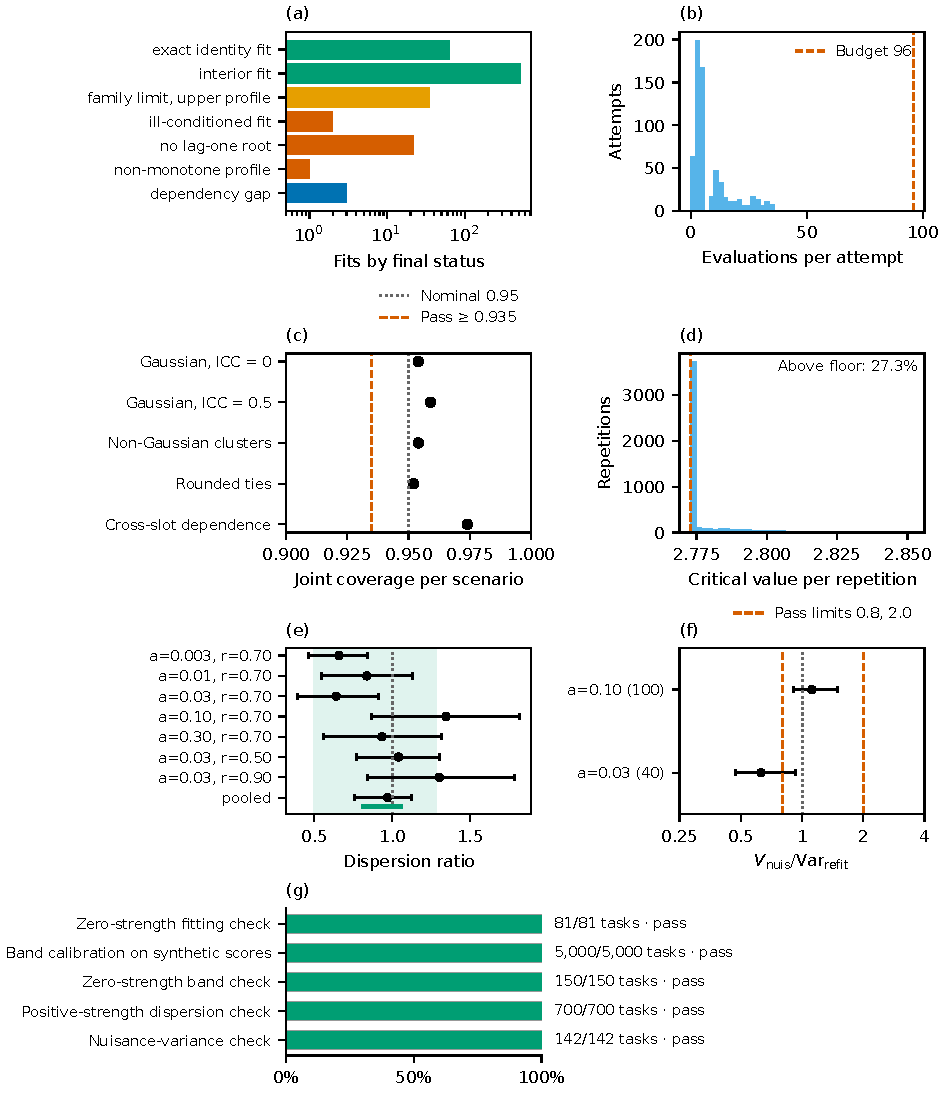
\includegraphics[width=\textwidth,height=150mm,keepaspectratio]{generated/J4_gate_diagnostics.pdf}
\caption{Validation-gate diagnostics from the public aggregates: (a) final fit statuses and (b) solver evaluations per attempt in the zero-strength fitting check (budget \resultnum{j.gate.solver_budget}{96}); (c) joint coverage per scenario and (d) critical values in the band calibration on synthetic scores, with the pass mark, nominal level and critical-value floor \resultnum{j.gate.critical_floor}{2.7729}; (e) dispersion ratios in the positive-strength dispersion check with bootstrap intervals and calibrated cell (shading) and pooled (green segment) thresholds; (f) local nuisance-variance estimates relative to full refits in the nuisance-variance check, with one-sided bounds; (g) completed tasks and verdict by stage. Family limits are gaps. The zero-strength band check uses its corrected aggregate record.}\label{fig:gate-diagnostics}
\end{figure}



\subsection{Execution, release and amendment v4.4}\label{sec:record-execution}\phantomsection\label{supp:execution-records}

\paragraph{Execution rules.}
The original operational deadline was 18 October 2026 at 23:59 America/Sao\_Paulo (19 October at 02:59 UTC). % M44 RC32
Eight shards executed the tiers in fixed order on a single host whose environment matched the one bound by the freeze record (see the article's Data and code availability statement; an operating-system update after the run changed that host's platform string, Section~\ref{sec:verification-limits}). AUC, band width or invalidity did not reorder them. % M44
The projected cost of the gate and all six tiers ranged from about 256 hours with measured costs to about 726 hours with 25\% retries. The latter exceeded the time between the freeze and the close, so tiers 3--6 could have been partial at the close, and their controls and sensitivities were not promised; in the event every tier finished (Section~\ref{sec:inventory}). % M80
At the close or release, each comparison/$r$ unit is recorded as not started, partial at the operational close, complete but invalid, or complete and valid, preserving attempts (Section~\ref{sec:inventory}). % M45
The main curve is valid only if all nine tier-1 units (B on the observed channel, one per $r$) are complete and valid in the released inventory. % M46
A tier-1 unit that is not started, partial or complete but invalid, for any reason, invalidates the main curve without deleting the boundaries of other units. Tier 1 therefore had to finish before the original deadline if early full-inventory release did not occur. % M46 RC33
The main curve could thus be invalidated by chance as well as by the clock. With a correct procedure and a critical value of at least 2.7729, the probability that one unit's $a=0$ band misses 0.5 is at most about 0.0056 under normal logit errors. If the nine B units are independent, the probability that at least one misses by chance alone is up to about 4.9\%. % M75

\paragraph{Release rule.}
A linked amendment registered on 28 September 2026, at the first author's instruction and before any tier started, permits release when all 414 units have final curve records and no curve worker is running, or at the original deadline; it permits no partial early release. Gate outcomes and curve estimates enter the results only through this release and its full inventory. % M85 RC34 M47
The frozen code remains revision \texttt{37513841}; the later release wrapper (Table~\ref{tab:record-identifiers}) implements this release rule without changing the grid, gates or inferential criteria. % M85 RC35 RC48
For an early release it passes the original deadline to the frozen release function, so the frozen record's close time keeps that conventional value. % M85 RC36 RC49
A separate release record supplies the actual release time, trigger, wrapper hash and released-output hash; the chronology needs both records. % M85 RC37

\paragraph{Shard incident and amendment v4.4.}
All five recorded gate stages passed, and the tiers started on 30 September 2026 (decision log item 114). On 1 October 2026 at 04:18 UTC, the worker of shard 5 ended during tier 2, and a relaunch with the frozen code failed in the same way. With the first author's authorization, the failure was reproduced on a copy of the unit outside the sealed store: in the cell at $a=0.003$ of the unit of D at $r=0.60$, the nuisance projection raised an ill-conditioned-local-profile error while propagating the nuisance, because the local profile Jacobian was degenerate, and the frozen runner does not handle that exception. Before this diagnosis, no tier-2 or later curve output had been read; only file counts, completion markers and modification times of that shard's units were inspected. % M89
Amendment v4.4, frozen in its own record, records a cell whose frozen execution ends with exactly that error, raised by the nuisance projection, as a sealed propagation gap with no attempt and with the hash of the successor runner that wrote it. Any other exception still ends the shard. The successor runner loads the frozen runner and runs its preflight and loop unchanged, replacing only the per-cell worker; it lives outside the frozen checkout, so the code hashes checked by the preflight and by shard resume are unchanged. A propagation gap follows the existing gap rules: at a positive strength it censors boundaries without invalidating the unit, and at $a=0$ it removes the zero-strength check. The inventory table reports it in its own column. % M89
The first author alone approved the amendment, the successor runner and the relaunch of the eight shards on 1 October at 14:33 UTC, during the second stage of the run: tier 1, the main curve against B, had finished and stayed sealed and unread, and no tier-2 or later curve output had been read. The amendment recorded that scientific ratification, with the supervisor's review, was still pending; it was covered by the ratification recorded later that day (decision log item 161), before the results became available. The shard resumed past its completed cells and recorded the gap at 14:35 UTC. Completed cells were not rerun. % M89
The rule applied to two cells, both at $a=0.003$ and $r=0.60$: the unit of D on the observed channel (\resultnum{v4.tab.T4.2-D-observed-main.gaps_propagation}{1} propagation gap) and the matching mobility unit of D (\resultnum{v4.tab.T4.3-D-observed-mobility.gaps_propagation}{1}). Its consequence for the reported results is confined to D at $r=0.60$: the first boundary against D there is censored at the propagation gap, $a=\resultnum{v4.tab.T1.D.r060.a_star.1}{0.003}$, while the next gap of that unit is a family limit at $a=\resultnum{j.models.D.r060.first.gap.1.a}{0.10}$, the first gap of D at seven of the other eight shares. Read after the results became available: below that family limit the point AUC against D stayed near 0.5 at $r=0.60$ (\resultnum{j.models.D.r060.a0100.auc}{0.506} at $a=0.01$ and \resultnum{j.models.D.r060.a0300.auc}{0.519} at 0.03), and every first and sustained boundary against D is censored at all nine shares (Section~\ref{sec:additional-models}), so the amendment moved the censoring point at that share without changing whether any comparison with D could be read. The sentence of the rule-assembled introduction that ``every reporting rule was fixed before any confirmatory result was released'' therefore holds only in this qualified sense: v4.4, an operational rule that decides how one kind of failure is recorded, was approved during the run, after the main curve had been computed and before any result was read or released.

\paragraph{Release chronology.}
% Moved from sections/results.tex (Release and unit inventory) of the rule-assembled attempt.
The results became available on \resultnum{v4.release.effective_local}{8 October 2026 at 11:26:02} America/Sao\_Paulo, triggered by \resultnum{v4.release.condition}{completion of the full inventory}; the nominal close was \resultnum{v4.protocol.close_local}{18 October 2026 at 23:59} America/Sao\_Paulo. The tiers ran in the fixed order, without changes based on AUC, band width or invalidity. No work was unfinished at release, so the declared-close rule did not have to stop any; only complete units contribute boundaries and AUC profiles (Section~\ref{sec:inventory}).

\subsection{Governance and ratification}\label{sec:record-governance}

The v1 protocol was frozen by the coordinating agent under the first author's delegation (decision log item 18), and the v4 decision specification records a delegated agent decision (decision log item 19); both records mark these decisions as pending ratification, and both took effect before that ratification. The authors ratified both, together with the later amendments and delegated decisions, on 1 October 2026, before the results became available (decision log item 161). % M83
The ratification record states the scope: v1 as history, v4 amended after partial exposure, amendment v4.4, the delegated decisions, the exploratory declarations and the interpretation rules; it records that acceptance of the released results could not be anticipated and is left to both authors' reading of the final manuscript. The release amendment of 28 September 2026 followed an explicit instruction of the first author; Section~\ref{sec:ai} describes the use of AI agents in these steps.

\clearpage
